 The proposed biomechanical model consist of two bodies, one representing the pectoral cage  and the second represents the breast soft tissues. Between the two bodies, a contact surface is defined in order to model tissues mechanics at the juncture interface.
 
The next sections describes the implementation of different interaction models that were tested during the implementation process. Since the breast tissues are attached to the pectoral muscle (Figure \ref{fig:contactsurface}), the contact surface was modeled using combinations of \textit{bonded} and \textit{no-separation frictional} interaction models.


\begin{figure}[!h]
\centering
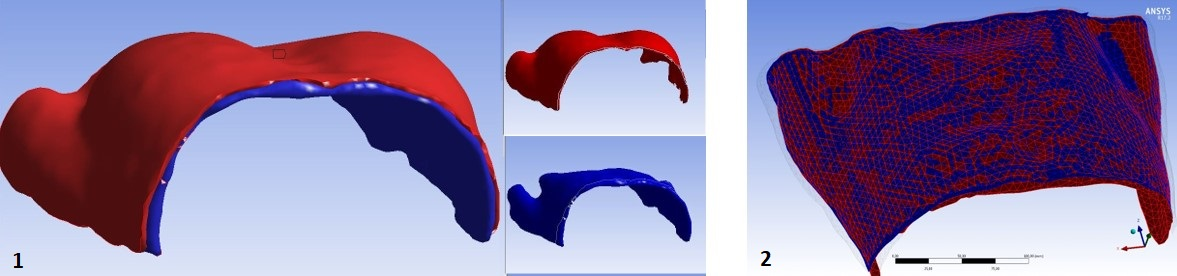
\includegraphics[width=0.9\textwidth,keepaspectratio]{figures/contactSurface.jpg} 
\caption{The two bodies representing the thoracic cage and breast with the associated contact surface.  Blue surface- the target surface, red surface - contact surface}
\label{fig:contactsurface}
\end{figure}

The results for pure bonded, no-separation sliding models as well as one combined contact surface are listed bellow, with their impact on global breast deformation. For some models partial results are presented, because of important solution instabilities  the deformed breast geometry is not available.  


\subsubsection*{Bonded contact surface}



\begin{figure}[!h]
\centering
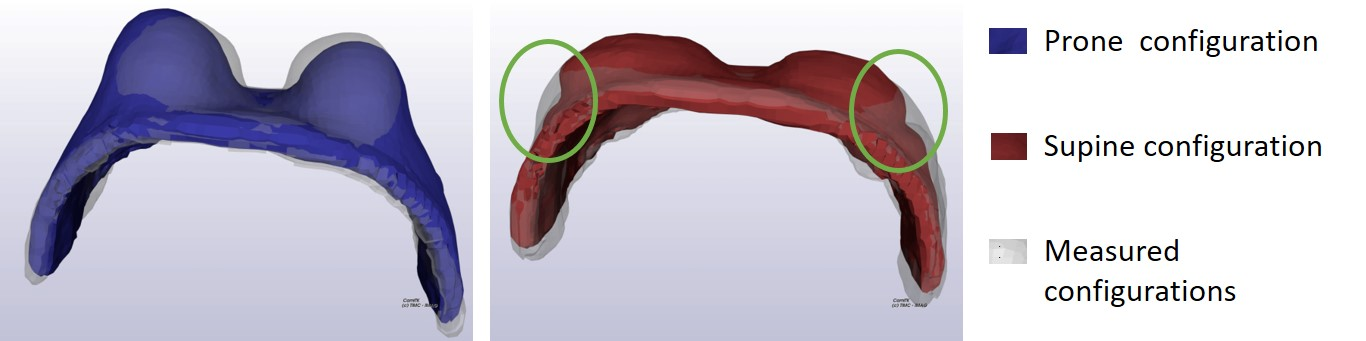
\includegraphics[width=0.9\textwidth,keepaspectratio]{figures/bondedcontact.jpg} 
\caption{Resulting breast deformation with a bonded contact model.}
\label{fig:bondedcontact}
\end{figure}

\subsubsection*{Sliding contact surface}

\begin{figure}[!h]
\centering
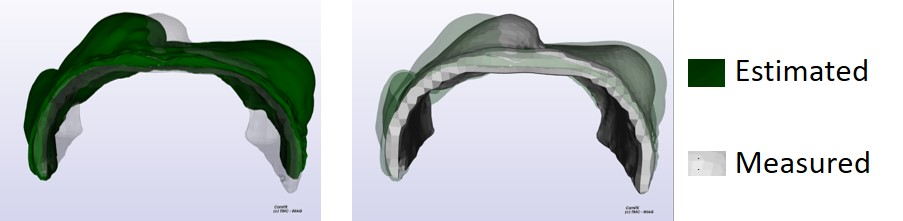
\includegraphics[width=0.9\textwidth,keepaspectratio]{figures/supinetilted_sliding.jpg} 
\caption{Resulting breast deformation in supine tilted configuration with a sliding contact model.}
\label{fig:bondedcontact}
\end{figure}

\subsubsection*{Mixt contact surface}

\begin{figure}[!h]
\centering
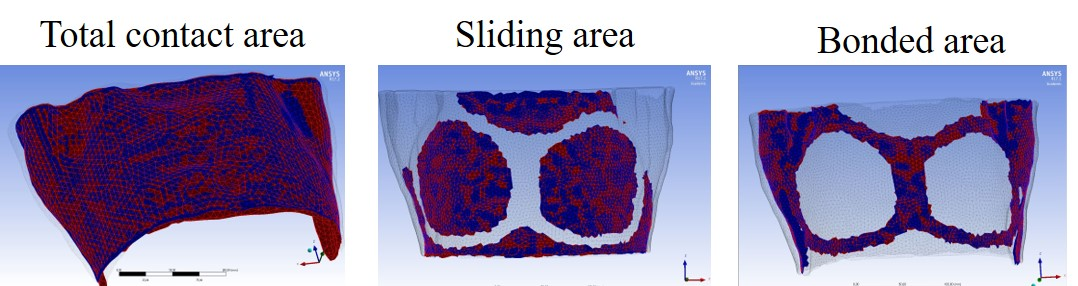
\includegraphics[width=0.9\textwidth,keepaspectratio]{figures/mixtcontactarea.jpg} 
\caption{The contact surface divided in two regions: sliding region and bonded region.}
\label{fig:bondedcontact}
\end{figure}
\subsubsection*{Sliding contact surface with ligaments}